\documentclass[10pt]{beamer}
\mode<presentation>
\usepackage{amssymb,textcomp}
%\usepackage{beamerthemesplit}
\usepackage{beamerthemeJuanLesPins}
\usepackage{verbatim}
\usepackage{algorithm2e}
\usefonttheme{serif}
\title{M\'etodos Iterativos para la Resoluci\'on Num\'erica de Sistemas de Ecuacionesl Lineales.}
\author{Jos\'e Luis Ram\'irez B.}
\date{\today}
\begin{document}
\frame{\titlepage}
%\section[Introducci\'on]{}
\frame{\tableofcontents}
\section{Introducci\'on}
\begin{frame}{Problemas de los m\'etodos directos para la resoluci\'on de (SL).}
  \begin{itemize}
   \item<1-> El m\'etodo de Gauss y sus variantes se conocen con el nombre de m\'etodos
   directos: se ejecutan un n\'umero finito de pasos y dan a lugar a una soluci\'on
   que ser\'ia exacta si no fuese por los errores de redondeo.
   \item <2->Cuando el tama\~no de la matriz $A$ es grande ($n >> 100$), la propagaci\'on del error de redondeo es tambi\'en grande, y los
  resultados obtenidos pueden diferir de los exactos.
  \end{itemize}
\end{frame}
  %%%%%%%
  \frame{
    \frametitle{Problemas de los m\'etodos directos para la resoluci\'on de (SL).}
    \begin{itemize}
      \item Muchas de las matrices que aparecen en (SL) poseen la mayor\'ia de sus elementos nulos. Estas matrices reciben el nombre de matrices dispersas o sparse.
      \begin{enumerate}
      \item<2-> Si los elementos no nulos est\'an distribuidos alrededor de la diagonal principal, son de aplicaci\'on todav\'ia los m\'etodos directos que conservan la estructura diagonal, como $LU$.
      \item<3-> Si no ocurre lo anterior, al aplicar m\'etodos directos se produce un fen\'omeno de llenado. Entonces, si no se realiza una adaptaci\'on de los m\'etodos directos los resultados no van a ser, en general, buenos.
      \end{enumerate}
    \end{itemize}
  }
  %%%%%%
  \section{M\'etodos Iterativos}
  \begin{frame}{M\'etodos Iterativo}
  \begin{itemize}
  \item<1-> Un m\'etodo iterativo que da resoluci\'on al sistema $Ax = b$ es aquel que genera, a partir de un vector inicial $x^{(0)}$, una sucesi\'on de vectores $x^{(1)},x^{(2)}, \ldots$.
  \item<2-> El m\'etodo se dir\'a que es consistente con el sistema $Ax = b$, si el l\'imite de dicha sucesi\'on, en caso de existir, es
  soluci\'on del sistema.
  \item<3-> Se dir\'a que el m\'etodo es convergente si la sucesi\'on generada por cualquier vector inicial $x^{(0)}$ es convergente a la soluci\'on del sistema.
  \item<4-> El vector $r^{(k)} = b-Ax^{(k)}$ es el vector residual obtenido en la $k$-\'esima iteraci\'on.
  \end{itemize}
  \end{frame}
  %%%%%%
  \begin{frame}{M\'etodos Iterativo}
  Si un m\'etodo es convergente es consistente, sin embargo, el rec\'iproco no es cierto.
  \uncover<2->{
  \begin{block}{Ejemplo:}
  El m\'etodo $x^{(n+1)} = 2x^{(n)} - A^{-1}b$ es consistente con el sistema $Ax = b$ pero no es convergente. En efecto:
  \end{block}}
  \end{frame}
  %%%%%%
  \begin{frame}{M\'etodos Iterativo}
  \begin{eqnarray}
  x^{(n+1)}-x & = & 2x^{(n)}-A^{-1}b-x = 2x^{(n)}-2x-A^{-1}b+x \nonumber\\
  & = & 2(x^{(n)}-x)-(A^{-1}b-x)\nonumber
  \end{eqnarray}
  y como $A^{-1}b = x$, se tiene que:
  \begin{block}{}
  $$
  x^{(n+1)}-x = 2(x^{(n)}-x)
  $$
  \end{block}
  \uncover<2->{
  Si existe \textcolor{red}{$\displaystyle\lim_{n \to \infty} x^{(n)} = x^*$}, se tiene que:
  \begin{block}{}
  $$
  x^* - x=2(x^* - x) \Rightarrow x^* - x =0 \Rightarrow x^* = x
  $$
  \end{block}
  es decir, el l\'imite es soluci\'on del sistema $Ax = b$, por lo que el m\'etodo es consistente.}
  \end{frame}
  %%%%%%
  \begin{frame}{M\'etodos Iterativo}
  Sin embargo, de $x^{(n+1)} - x = 2(x^{(n)} - x)$ se obtiene que:
  \begin{block}{}
  $$
  \|x^{(n+1)}-x\| = 2\|x^{(n)}-x\|
  $$
  \end{block}
  es decir, el vector $x^{(n+1)}$ dista el doble de lo que distaba $x^{(n)}$, por lo que el m\'etodo no puede ser convergente.
  \end{frame}  
  %%%%
  \section{Refinamiento Iterativo}
  \begin{frame}{Refinamiento Iterativo}
    \begin{itemize}
      \item Al resolver un sistema de ecuaciones $Ax = b$ utilizando un m\'etodo num\'erico
      se obtiene una aproximaci\'on $\tilde x$ de la verdadera soluci\'on del sitema.
      \item<2-> La exactitud de dicha soluci\'on depende de errores inherentes a los c\'alculos realizados.
      \item<3-> Sea $x$ la soluci\'on exacta del sistema y $\tilde x$ es la aproximaci\'on, por lo tanto cuando se sustituye $\tilde x$ en el sistema se obtiene:
      \begin{block}{}
      $$
      A\tilde x \approx b
      $$
      \end{block}
      esto significa que al realizar la resta $b - A\tilde x \neq 0$      
    \end{itemize}
  \end{frame}
  %%%%%
  \begin{frame}{Refinamiento Iterativo}
    \begin{itemize}      
      \item Definiendo a esta diferencia $r$ (residuo), as\'i $r = b - A\tilde x$.
      \item<2-> La soluci\'on deseada es
      de la forma $\tilde x + z$ tal que al sustituir en el sistema de ecuaciones se obtenga
      $$
      A(\tilde x + z) = b
      $$
      y desarrollando se obtiene
      \begin{eqnarray}
        \uncover<3->{\nonumber A(\tilde x + z) & = & b}\\
        \uncover<4->{\nonumber A\tilde x + Az & = & b}\\
        \uncover<5->{\nonumber Az & = & b - A\tilde x}\\
        \uncover<6->{\nonumber Az & = & r}
      \end{eqnarray}
      \item<7-> Una vez que obtenida $z$ se puede
      crear una mejor aproximación $\tilde x + z$ de la soluci\'on.
    \end{itemize}
  \end{frame}
  %%%%%%
  \begin{frame}
    \frametitle{Ejemplo:}
    Al resolver el sistema Ax = b donde
    $$
    A = \left[\begin{array}{ccc}
      60 & 30 & 20\\
      30 & 20 & 15\\
      20 & 15 & 12
    \end{array}\right] \quad \text{ y } \quad b = \left[\begin{array}{c}
      110\\
      65\\
      47
    \end{array}\right]
    $$
    suponiendo que una soluci\'on aproximada es $b = \left[\begin{array}{c}
      0.9\\
      0.8\\
      1.2
    \end{array}\right]$
  \end{frame}
  %%%%%%
  \begin{frame}
    \frametitle{Ejemplo:}
    \begin{itemize}
    \item Aplicando un paso de refinamiento iterativo tomando $tol = 10^{-5}$, se tendr\'ia que:
    $$
    x^{(0)} = \left[\begin{array}{c}
      0.9\\
      0.8\\
      1.2
    \end{array}\right]
    $$
    \item<2-> Calculando el residuo $r^{(0)} = b - Ax^{(0)} = \left[\begin{array}{c}
      8\\
      4\\
      2.6
    \end{array}\right]$
    \item<3->Verificando criterio de parada $\|r^{(0)}\|_{\infty} = 8 > tol$
  \end{itemize}
  \end{frame}
  %%%%%%
  \begin{frame}
    \frametitle{Ejemplo:}
    \begin{itemize}
      \item Obteniendo $z$ resolviendo el sistema $Az = r$ se obtiene $z =\left[\begin{array}{c}
        0.1\\
        0.2\\
        -0.2
      \end{array}\right]$
      \item<2->Generando la nueva aproximaci\'on
      $$
      x^{(1)} = x^{(0)} + z = \left[\begin{array}{c}
        0.9\\
        0.8\\
        1.2
      \end{array}\right] + \left[\begin{array}{c}
        0.1\\
        0.2\\
        -0.2
      \end{array}\right] = \left[\begin{array}{c}
        1\\
        1\\
        1
      \end{array}\right]
      $$
      \item<3-> Calculando el residuo $r^{(1)} = b - Ax^{(1)} = \left[\begin{array}{c}
        -0.14210854715202\\
        0\\
        0
      \end{array}\right]\times 10^{-13}$
    \end{itemize}
  \end{frame}
  %%%%%%
  \begin{frame}
    \frametitle{Ejemplo:}
    \begin{itemize}
      \item Verificando criterio de parada $\|r^{(1)}\|_{\infty} = 0.14210854715202\times 10^{-13} < tol$
      \item<2->Seg\'un el criterio de parada la mejor aproximaci\'on es $x=\left[\begin{array}{c}
        1\\
        1\\
        1
      \end{array}\right]$
    \end{itemize}
  \end{frame}
  %%%%%%}
  \begin{frame}
    \frametitle{Refinamiento Iterativo}
    \begin{itemize}
      \item Si suponemos que la soluci\'on aproximada al sistema lineal $A x = b$ se determina usando aritm\'etica de $t$ d\'igitos, se puede demostrar que el vector residual $r$ para la aproximaci\'on $\tilde x$ tiene la propiedad
      $$
       \|r\| = 10^{-t}\|A\|\|\tilde x\|
      $$
      \item<2-> De esta ecuaci\'on aproximada, se puede obtener una estimaci\'on del n\'umero de condici\'on efectivo para la aritm\'etica de $t$ d\'igitos, sin la necesidad de invertir la matriz $A$.
    \end{itemize}
  \end{frame}
  %%%%%%
  \begin{frame}
    \frametitle{Refinamiento Iterativo}
    \begin{itemize}
      \item La aproximaci\'on del n\'umero de condici\'on $\kappa(A)$ a $t$ d\'igitos viene de considerar el sistema lineal $A z = r$.
      \item<2-> De hecho $\tilde z$, la soluci\'on aproximada de $A z = r$, satisface que      
      $$
       \tilde z \approx A^{-1}r = A^{-1}(b-A\tilde x) = A^{-1}b - A^{-1}A\tilde x = x - \tilde x
      $$
      \item<3-> as\'i que $\tilde z$ es una estimaci\'on del error cometido al aproximar la soluci\'on del sistema original.      
      \begin{eqnarray}
       \nonumber \|\tilde z\| & \approx & \|x-\tilde x\|=\|A^{-1}r\| \leq \|A^{-1}\|\|r\|\\
       \nonumber & \approx & \|A^{-1}\|\left(10^{-t}\|A\|\|\tilde x\|\right) = 10^{-t}\|\tilde x\|\kappa(A)
      \end{eqnarray}
      \item<4-> Esto proporciona una aproximaci\'on para el n\'umero de condici\'on involucrado en la soluci\'on del sistema $A x = b$ usando $t$ d\'igitos:
      $$
       \kappa(A) \approx 10^t\frac{\|\tilde z\|}{\|\tilde x\|}
      $$      
    \end{itemize}
  \end{frame}      
  %%%%%%
  \begin{frame}
    \frametitle{Ejemplo:}
    \begin{itemize}
      \item<1->El sistema lineal $A x = b$ dado por
      $$
      \left(\begin{array}{ccc}
          3.333 & 15920 & -10.333\\
          2.222 & 16.71 & 9.612\\
          1.5611 & 5.1791 & 1.6852
        \end{array}\right)\left(\begin{array}{c}
        x_1\\
        x_2\\
        x_3
        \end{array}\right)=\left(\begin{array}{c}
        15913\\
        28.544\\
        8.4254
        \end{array}\right)
      $$      
      tiene la soluci\'on exacta $x = (1, 1, 1)^t$
      \item<2-> Usando eliminaci\'on Gaussiana y aritm\'etica de redondeo de 5 d\'igitos a
      $$
      \left(\begin{array}{ccc|c}
             3.333 & 15920 & -10.333 & 15913\\
             0 & -10596 & 16.501 &-10580\\
             0 & 0 & -5.079 & -4.7
            \end{array}\right)
      $$
      
      La soluci\'on aproximada a este sistema es
      
      $$
      \tilde x^{(0)} = (1.2001; 0.99991; 0.92538)^t
      $$
      \end{itemize}
\end{frame}
  %%%%%%
  \begin{frame}
    \frametitle{Ejemplo:}
    \begin{itemize}
      \item El vector residual correspondiente a $\tilde x$ calculado con doble precisi\'on (y luego redondeado a cinco d\'igitos) es 
      \small{
      \begin{eqnarray}
       \nonumber r^{(0)} & = & b - A \tilde x^{(0)} =\\
       \nonumber   & = & \left(\begin{array}{c}
            15913\\
            28.544\\
            8.4254
            \end{array}\right) - \left(\begin{array}{ccc}
             3.333 & 15920 & -10.333\\
             2.222 & 16.71 & 9.612\\
             1.5611 & 5.1791 & 1.6852
            \end{array}\right)\left(\begin{array}{c}
            1.2001\\
            0.99991\\
            0.92538
            \end{array}\right)\\
      \nonumber & = & \left(\begin{array}{c}
            -0.0051818\\
            0.27413\\
            -0.18616
            \end{array}\right)
      \end{eqnarray}}
      
      \item<2-> as\'i que 
       $$
       \|r^{(0)}\|_{\infty} = 0.27413
       $$
      \end{itemize}
    \end{frame}
  %%%%%%
  \begin{frame}
    \frametitle{Ejemplo:}
    \begin{itemize}
      \item<1-> La estimaci\'on del n\'umero de condici\'on se obtiene resolviendo primero el sistema $A z^{(0)} = r$:      
      $$
      \left(\begin{array}{ccc}
             3.333 & 15920 & -10.333\\
             2.222 & 16.71 & 9.612\\
             1.5611 & 5.1791 & 1.6852
            \end{array}\right)\left(\begin{array}{c}
            z_1\\
            z_2\\
            z_3
            \end{array}\right)=\left(\begin{array}{c}
          -0.0051818\\
          0.27413\\
          -0.18616
            \end{array}\right)
      $$
      \item <2-> La soluci\'on $z^{(0)} = (-0.20008; 8.9989 \times 10^{-5}; 0.074607)^t$ Usando la estimaci\'on del n\'umero de condici\'on      
       $$
       \kappa(A) \approx 10^5\frac{\|\tilde z^{(0)}\|_{\infty}}{\|\tilde x^{(0)}\|_{\infty}} = \frac{10^5(0.20008)}{1.2001} = 16672
       $$
      \end{itemize}
    \end{frame}  
  %%%%%%
  \begin{frame}
    \frametitle{Ejemplo:}
    \begin{itemize}
      \item Calculado $\tilde z^{(0)}$ se puede generar la nueva aproximaci\'on $\tilde x^{(1)}$
      $$
      \tilde x^{(1)} = \tilde x^{(0)} + \tilde z^{(0)} = (1.0000; 1.0000; 0.99999)^t
      $$
      \item<2-> y el error real en esta aproximaci\'on es
      $$
      \|x - \tilde x^{(1)}\|\infty = 1.0 \times 10^{-5}
      $$
      \item<3-> calculando $r^{(1)} = b - A \tilde x^{(1)}$, y resolviendo el sistema $A z^{(1)} = r^{(1)}$, se obteniene
      $$
      \tilde z^{(1)} = (-2.7003 \times 10^{-8}; 1.2973 \times 10^{-8}; 9.9817 \times 10^{-6})^t
      $$
      \item<4-> Puesto que $\|\tilde z^{(1)}\| \leq 10^{-5}$, se concluye que
      $$
      \tilde x^{(2)}= \tilde x^{(1)} + \tilde z^{(1)} = (1.0000; 1.0000; 1.0000)^t
      $$      
      es suficientemente preciso.
    \end{itemize}
  \end{frame}
  %%%%%%
  \begin{frame}
    \frametitle{Ejemplo:}
    \begin{itemize}
      \item<1-> Se ha usado la estimaci\'on $\tilde z \approx x - \tilde x$, donde $\tilde z$ es la soluci\'on aproximada al sistema $A z = r$.
      \item<2-> A partir de este resultado, se genera la nueva aproximaci\'on $\tilde x + \tilde z$.
      \item<3-> Este proceso puede ser repetido para refinar la soluci\'on sucesivamente hasta alcanzar convergencia.
    \end{itemize}
  \end{frame}
  %%%%%  
  \begin{frame}    
    \frametitle{Algoritmo}
    \small
\begin{algorithm}[H]
 \SetKwInOut{Input}{input}
 \SetKwInOut{Output}{output}
 \caption{Algoritmo de Refinamiento Iterativo.}
 \Input{$A \in \mathbb{R}^{n \times n}$, $b \in \mathbb{R}^n$, N\'umero m\'aximo de iteraciones $N$, tolerancia $TOL$.}
 \Output{Soluci\'on aproximada $x\in\mathbb{R}^n$.}
 \BlankLine
 Resolver $Ax=b$\\
 \For{$k\leftarrow 1$ \KwTo $N$}
 {
  $r=b-Ax$\\
  Resolver $Ay=r$ (usando eliminaci\'on Gaussiana en el mismo orden que en el paso 1).\\
  Calcular $K(A) = 10^t\displaystyle\frac{\|y\|}{\|x\|}$ (solo se calcula la primera vez).\\
  $x=x+y$\\
  \If{$\|y\|<TOL$}
  {
    salida $x$\\
    parar
  }
 }
\end{algorithm}
  \end{frame}
  %%%%%%
  \section{M\'etodos Iterativos de Punto Fijo}
  \begin{frame}{Esquemas de Punto Fijo}
    Supongase un (SL) $Ax = b$, se busca una matriz $T \in \mathcal{M}_n$ y un vector $c \in \mathbb{R}^{n}$, de forma que la matriz $I - T$ sea inversible y que la \'unica soluci\'on del sistema lineal
\begin{block}{}
$$
 \underbrace{x=Tx+c}_{(I-T)x=c}
 $$
\end{block}
es la soluci\'on  de $Ax=b$.
\end{frame}    
%%%%%%
\begin{frame}{Esquemas de Punto Fijo}
  Considerando $x^{(0)} \in \mathbb{R}^{n}$ un vector arbitrario, se construye una sucesi\'on de vectores $\{x\}_{k=0}^{\infty}$ dada por
  \begin{block}{}
   $$
   x^{(k+1)} = Tx^{(k)}+c; \qquad k \in \mathbb{N}\cup \{0\}
   $$
  \end{block}
  y se pretende que la sucesi\'on $\{x\}_k$ converja a la soluci\'on del sistema lineal.
  \end{frame}
  %%%%%%  
  \begin{frame}{Esquemas de Punto Fijo}
    \begin{block}{Definici\'on}
    El m\'etodo iterativo $x^{(k+1)} = Tx^{(k)} + c$ es convergente si existe un vector $x \in \mathbb{R}^n$ tal que:
    $$
    \lim_{k\rightarrow\infty}x^{(k)} = x
    $$
    para cualquier vector inicial $x^{(0)} \in \mathbb{R}^n$. En ese caso,
    $$
    x = Tx + c
    $$
    \end{block}
    \end{frame}
    %%%%%%
    \begin{frame}{Criterio de Convergencia}
    El error en cada iteraci\'on se puede medir, por tanto como:
    \uncover<2->{
    \begin{block}{}
    $$
    e^{(k)} = x^{(k)} - x
    $$
    \end{block}}
    \uncover<3->{Se tiene que:}
    \begin{eqnarray}
    \uncover<4->{e^{(k)} = x^{(k)} - x & = & (Tx^{(k-1)} + c) - (Tx + c) = T(x^{(k-1)} - x) =\nonumber\\}
    \uncover<5->{&&Te^{(k-1)} =  \cdots = T^ke^{(0)}\nonumber\\}
    \uncover<6->{&&\Rightarrow e^{(k)} = T^ke^{(0)}\nonumber}
    \end{eqnarray}
    \uncover<7->{De ese modo, el error en las iteraciones depende de las potencias sucesivas de la matriz $T$, lo que dar\'a el criterio para la convergencia del M\'etodo Iterativo.}
    \end{frame}
    %%%%%%
    \begin{frame}{Criterio de Convergencia}
    \begin{itemize}
    \item<1-> Se mostr\'o por inducci\'on que
    $$
    e^{(k)} = T^ke^{(0)}
    $$
    \item<2-> Entonces $e^{(k)} \to 0$ para todo $e^{(0)}$ si y s\'olo si $ T^k \to 0$.
    \begin{block}{}
    $$
     \lim_{k \to \infty}\|e^{(k)} \| \to 0 \quad sii \quad \lim_{k \to \infty}\|T^k\| \to 0
     $$
    \end{block}
    \item<3-> Si $T$ es una matriz diagonalizable, exiten matrices $P$ y $\Lambda$, tales que $T=P\Lambda P^{-1}$, donde $\Lambda$ es una matriz diagonal con los autovalores de $T$ en la diagonal.
    \begin{eqnarray}
     T & = & P \Lambda P^{-1}\nonumber\\
     T^{k} & = & P \Lambda P^{-1}P \Lambda P^{-1}\cdots P \Lambda P^{-1}\nonumber\\
     T^{k} & = & P \Lambda^{k} P^{-1}\nonumber
    \end{eqnarray}
    \end{itemize}
    \end{frame}
    %%%%%%
    \begin{frame}{Criterio de Convergencia}
    \begin{itemize}
     \item<1-> Donde
     $$
     \Lambda^{k} = \left(\begin{array}{cccc}
                          \lambda_1^{k} & & & \\
                          & \lambda_2^{k} & & \\
                          & & \ddots & \\
                          & & & \lambda_n^{k}
                         \end{array}\right)
     $$
     \item<2-> De esta manera
     \begin{block}{}
     \begin{eqnarray}
        \lim_{k \to \infty}\|T^{k}\| \to 0 & \Rightarrow & \lim_{k \to \infty}\|P \Lambda^{k} P^{-1}\| \to 0 \Rightarrow \lim_{k \to \infty}\|\Lambda^{k}\| \to 0\nonumber\\
         & \Rightarrow & \lim_{k \to \infty}|\lambda_i^{k}| \to 0 \Rightarrow |\lambda_i|<1\quad i=1,2,\ldots,n\nonumber
     \end{eqnarray}
     \end{block}
    \end{itemize}
    \end{frame}
    %%%%%%
    \begin{frame}{Criterio de Convergencia}
    \begin{itemize}
     \item Si la magnitud de todos los autovalores de la matriz de iteraci\'on $T$ son menores que 1, entonces el esquema iterativo es convergente.
     \uncover<2->{\begin{block}{Teorema}
                   Un esquema iterativo definido por $x^{(k+1)} = Tx^{(k)}+c$ es convergente si y s\'olo si $\rho(T) < 1$.
                  \end{block}}
     \item<3-> Es m\'as sencillo calcular la norma de una matriz que el c\'alculo de sus autovalores
     $$
     \left.\begin{array}{lcl}
            Tx & = & \lambda x \\
            \|Tx\| & = & |\lambda|\|x\|\\
            \|Tx\| & \leq & \|T\|\|x\|
           \end{array}\right\} \Rightarrow |\lambda|\|x\| \leq \|T\|\|x\| \Rightarrow |\lambda| \leq \|T\|
     $$
     \uncover<4->{Por lo que una condici\'on suficiente para la convergencia es: \textcolor{red}{$\|T\| < 1$}}
    \end{itemize}
    \end{frame}
    %%%%%%
    \begin{frame}{Tasa de Convergencia}
    \begin{itemize}
    \item<1-> En el dise\~no de un m\'etodo iterativo, adem\'as de asegurar la consistencia y convergencia del m\'etodo, es importante el concepto de velocidad de convergencia.
    \item<2-> Supongase que se tiene una aproximaci\'on de la soluci\'on, $x^{(k)}$ con $q$ cifras significativas,
    $$
    \|e^{(k)}\| \leq \frac{1}{2}10^{-q}\|x\|
    $$
    \item<3-> y se desea saber cu\'antas iteraciones m\'as se tienen que hacer para obtener $m$ cifras correctas m\'as. Interesa, por lo tanto, saber cu\'antas iteraciones $N$ hay que hacer para que,
    $$
    \|e^{(k+N)}\| \leq \frac{1}{2}10^{-(q+m)}\|x\|
    $$
    es decir
    \begin{block}{}
     $$
    \|e^{(k+N)}\| \leq 10^{-m}\|e^{(k)}\|
    $$
    \end{block}
    \end{itemize}
    \end{frame}
    %%%%%
    \begin{frame}{Tasa de Convergencia}
    \begin{itemize}
     \item<1-> Esto permitir\'a dar informaci\'on sobre la velocidad con que la sucesi\'on de aproximaciones $x^{(k)}$ se acerca a la soluci\'on.
     \item<2-> Se sabe que $e^{(k+N)} = T^{N}e^{(k)}$, que tomando norma es
     $$
     \|e^{(k+N)}\| \leq \|T^{N}\|\|e^{(k)}\|
     $$
     \item<3-> De manera que para conseguir las $m$ cifras significativas es suficiente exigir que $\|T^{N}\| \leq 10^{-m}$ o, equivalentemente
     $$
     -\log_{10}\|T^{N}\| \geq m
     $$
     \item<4-> As\'i, para conseguir $m$ cifras significativas es suficiente hacer $N$ iteraciones con
     $$
     N \geq \frac{m}{R}
     $$
    \end{itemize}
    \end{frame}
    %%%%%%%
    \begin{frame}{Tasa de Convergencia}
    \begin{itemize}
     \item Donde $R$ se define como:
     $$
     R = -\frac{1}{N}\log_{10}\|T^{N}\| = -\log_{10}\left(\|T^{N}\|^{1/N}\right)
     $$
     \item El par\'ametro $R$ se puede interpretar como la velocidad de convergencia: cuanto mayor es $R$ menos iteraciones hay que hacer para incrementar la precisi\'on en la aproximaci\'on.
     \item Se puede comprobar que
     $$
     \lim_{N \to \infty}\|T^{N}\|^{1/N} = \rho(T)
     $$
     por lo tanto, la velocidad asint\'otica de convergencia del m\'etodo es
     $$
     R_{\infty} = \log_{10}\left(\frac{1}{\rho(T)}\right)
     $$
     \end{itemize}
    \end{frame}
    %%%%%%
    \begin{frame}{Tasa de Convergencia}
    \begin{itemize}
     \item<1-> El radio espectral hace el papel del factor asint\'otico de convergencia del m\'etodo.
     \item<2-> Para $\rho(T) \simeq 0$, la velocidad de convergencia $R_{\infty}$ es muy grande y el m\'etodo tiene una convergencia muy r\'apida.
     \item<3-> Para $\rho(T) = 1 - \varepsilon$, con $\varepsilon \simeq 0$ positivo, la velocidad de convergencia es positiva pero peque\~na y el m\'etodo converge pero lo hace lentamente.
     \item<4-> En cambio, si $\rho(T) > 1$ la velocidad de convergencia es negativa por lo que la convergencia no est\'a asegurada.
    \end{itemize}
    \end{frame}
    %%%%%   
    \begin{frame}{Construcci\'on de los M\'etodos}
      Considerando la descomposici\'on
      $$
      A = M-N, \quad M \mbox{ regular }
      $$
      \uncover<2->{
      El sistema $Ax=b$ se puede escribir en la forma
      $$
      Mx = Nx+b,\mbox{ es decir, } x = M^{-1}Nx + M^{-1}b
      $$
      lo que sugiere el esquema iterativo}
      \uncover<3->{
      \begin{block}{}
      $$
      x^{(k+1)}=M^{-1}Nx^{(k)} + M^{-1}b
      $$
      \end{block}
      donde $T=M^{-1}N$ y $c=M^{-1}b=(I-T)A^{-1}b$, por lo que el m\'etodo as\'i construido es consistente con el sistema.}
      \end{frame}
      %%%%%
      \begin{frame}{Construcci\'on de los M\'etodos}
      \begin{itemize}
       \item El esquema anterior tamb\'en es esquivalente a
      \begin{block}{}
       $$
       x^{(k+1)} = x^{(k)} + M^{-1}(b-Ax^{(k)})
       $$
      \end{block}
      donde $r^{(k)} = b-Ax^{(k)}$ es el residual de la $k$-\'esima iteraci\'on y $M$ es un precondicionador del sistema.
      \item<2-> En lo sucesivo se considera la descomposici\'on aditiva de la matriz $A$ como
      \begin{center}
      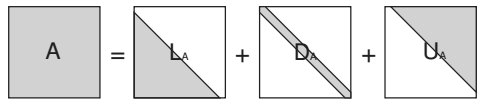
\includegraphics[scale=0.5]{descomA.png}
      \end{center}
      donde $L_A$ es la parte triangular inferior de la matriz sin incluir la diagonal, $D_A$ es la diagonal de $A$, y $U_A$ es la parte triangular superior sin incluir la diagonal.
      \end{itemize}
      \end{frame}
      %%%%%%
      \subsection{M\'etodo de Jacobi}      
      \begin{frame}{M\'etodo de Jacobi}
      \begin{itemize}
       \item Se basa en una descomposici\'on de la matriz $A$ del tipo $A = M - N$ , con $M = D$, parte diagonal de la matriz $A$, y $N = L + U$
       \item<2-> Obliga a resolver un sistema diagonal en cada paso.
       \item <3-> De esta manera queda que $A=D-L-U=D-(L+U)$, por lo tanto el sistema se transforma en:       
       $$
       Ax=b \Leftrightarrow (D-(L+U))x=b \Leftrightarrow Dx=(L+U)x + b
       $$
       \end{itemize}
      \end{frame}
      %%%%%%
      \begin{frame}{M\'etodo de Jacobi}
      \begin{itemize}
        \item<1-> As\'i, se calcula la soluci\'on del sistema, como el l\'imite de la sucesi\'on $\{x^{(k)}\}_{k \in N}$ donde se define el t\'ermino $(k+1)$-\'esimo como:
       
       $$
       x^{(k+1)}= D^{-1}(L+U)x^{(k)} + D^{-1}b
       $$
       
       siendo as\'i su matriz de iteraci\'on:
       
       $$
       T=D^{-1}(L+U)
       $$
       
       Entonces el sistema ha sido escrito como un proceso iterativo de la forma
       $$
       x^{(n+1)}= Tx^{(n)}+c .
       $$
      \end{itemize}
      \end{frame}
      %%%%%%       
      \begin{frame}{M\'etodo de Jacobi}
      \begin{itemize}
       \item<1-> Dado un sistema de ecuaciones:
       $$
       \left\{\begin{array}{c}
               a_{1,1}x_1 + a_{1,2}x_2 + \cdots + a_{1,i}x_i + \cdots + a_{1,n}x_n = b_1\\
         a_{2,1}x_1 + a_{2,2}x_2 + \cdots + a_{2,i}x_i + \cdots + a_{2,n}x_n = b_2\\
                   \vdots\\
         a_{i,1}x_1 + a_{i,2}x_2 + \cdots + a_{i,i}x_i + \cdots + a_{i,n}x_n = b_i\\
                   \vdots\\
         a_{n,1}x_1 + a_{n,2}x_2 + \cdots + a_{n,i}x_i + \cdots + a_{n,n}x_n = b_n
              \end{array}
       \right.
       $$
      \end{itemize}
    \end{frame}
    %%%%%%
    \begin{frame}{M\'etodo de Jacobi}
    \begin{itemize}
      \item<1->Si $a_{i,i}\neq 0$ para todo $i=1,\ldots,n$, entonces despejando $x_i$ de la $i$-\'esima ecuaci\'on, obtenemos el sistema equivalente       
       $$
       x_i = -\sum_{j=1,j\neq i}^n\left(\frac{a_{i,j}}{a_{i,i}}\right)x_j + \frac{b_i}{a_{i,i}}, \qquad i=1,\ldots,n
       $$       
       \item<2->Conocido $x^{(k-1)}$, se calcula la aproximaci\'on $x^{(k)}$, mediante la f\'ormula:       
       $$
       x_i^{(k)} = \displaystyle\frac{b_i-\displaystyle\sum_{j=1,j\neq i}^na_{i,j}x_j^{(k-1)}}{a_{i,i}}, \qquad i=1,\ldots,n
       $$       
       que es llamada f\'ormula escalar de iteraci\'on del m\'etodo de Jacobi.
      \end{itemize}
      \end{frame}     
      %%%%%%
      \begin{frame}{Ejemplo:}      
      Resolver el sistema de ecuaciones
      $$
\left(\begin{array}{ccc}
       4 & 1 & 0\\
       1 & 4 & 1\\
       0 & 1 & 4
      \end{array}\right)\left(\begin{array}{c}
      x_1\\
      x_2\\
      x_3
      \end{array}\right)=\left(\begin{array}{c}
      -3\\
      10\\
      1
      \end{array}\right)
      $$
      cuya soluci\'on es el vector

$$
\left(\begin{array}{c}
      x_1\\
      x_2\\
      x_3
      \end{array}\right)=\left(\begin{array}{c}
      -1.5\\
      3\\
      -0.5
      \end{array}\right)
$$
      y tomando como vector inicial $x^{(0)} = \left(\begin{array}{c}
      -1\\
      4\\
      -1
      \end{array}\right)$
      \end{frame}
      %%%%%%
      \begin{frame}{Ejemplo:}
        Procedamos a realizar la descomposici\'on de la matriz del sistema:
        \small{
        $$
        M=D=\left(\begin{array}{ccc}
               4 & 0 & 0\\
               0 & 4 & 0\\
               0 & 0 & 4
              \end{array}\right) \quad L=\left(\begin{array}{ccc}
               0 & 0 & 0\\
               -1 & 0 & 0\\
               0 & -1 & 0
              \end{array}\right) \quad U=\left(\begin{array}{ccc}
               0 & -1 & 0\\
               0 & 0 & -1\\
               0 & 0 & 0
              \end{array}\right)
        $$}           
        con        
        $$
        N=L+U
        $$
        Para comprobar si estamos convergiendo a la soluci\'on tomaremos elvalor de la norma del residuo $r^{(k)} = b - Ax^{(k)}$.
        $$        
        r^{(0)}	=b-Ax^{(0)} = \left(\begin{array}{c}
        -3\\
        -4\\
        1
        \end{array}\right) \Rightarrow \|r^{(0)}\|_\infty = 4
        $$
      \end{frame}   
      %%%%%%
      \begin{frame}{Ejemplo:}     
        El primero paso del esquema vendr\'ia dado por:
        $$
        Dx^{(1)} = N x^{(0)} + b = (L + U )x^{(0)} + b
        $$
        $$
\left(\begin{array}{ccc}
       4 & 0 & 0\\
       0 & 4 & 0\\
       0 & 0 & 4
      \end{array}\right)x^{(1)}=\left(\begin{array}{ccc}
       0 & -1 & 0\\
       -1 & 0 & -1\\
       0 & -1 & 0
      \end{array}\right)\left(\begin{array}{c}
      -1\\
      4\\
      -1
      \end{array}\right)+\left(\begin{array}{c}
      -3\\
      10\\
      1
      \end{array}\right)
      $$
      Y al resolver el sistema diagonal:
$$
x^{(1)} = \left(\begin{array}{c}
      -1.75\\
      3\\
      -0.75
      \end{array}\right)
$$
Con vector residual
$$
r^{(1)} = \left(\begin{array}{c}
      1\\
      0.5\\
      1
      \end{array}\right) \Rightarrow \|r^{(1)}\|_\infty = 1
$$
      \end{frame}
      %%%%%%
      \begin{frame}{Ejemplo:}
        Por tanto, el residuo ha disminuido. Si seguimos iterando:
        \begin{eqnarray}
          \nonumber x^{(2)} = \left(\begin{array}{c}
               -1.5\\
               3.125\\
               -0.5
               \end{array}\right) \quad \|r^{(2)}\|_\infty=0.5 \\
          \nonumber x^{(3)} = \left(\begin{array}{c}
               -1.5312\\
               3.0000\\
               -0.50312
               \end{array}\right) \quad \|r^{(3)}\|_\infty=0.125\\
               \nonumber x^{(4)} = \left(\begin{array}{c}
                -1.5\\
                3.0156\\
                -0.5
                \end{array}\right) \quad \|r^{(4)}\|_\infty=0.0625 \\
           \nonumber x^{(5)} = \left(\begin{array}{c}
                -1.5039\\
                3.0000\\
                -0.5039
                \end{array}\right) \quad \|r^{(5)}\|_\infty=1.5625e-02
         \end{eqnarray}
      \end{frame}        
      %%%%%%
      \begin{frame}
      \frametitle{M\'etodo de Jacobi}
      \begin{itemize} 
      \item<1-> El siguiente teorema de convergencia se refiere a un tipo de matrices.
      \end{itemize}
      \uncover<2->{
      \begin{block}{Teorema}
      Supongamos que una matriz $A$ sea diagonal estrictamente dominante:
      $$|a_{i,i}| >\sum_{j \neq i}|a_{i,j}|,\quad i = 1,\ldots, n$$
      Entonces, el m\'etodo de Jacobi converge para esta matriz.
      \end{block}}
      \end{frame}
      %%%%%%
      \begin{frame}
      \frametitle{M\'etodo de Jacobi}
      \begin{itemize}
      \item<1-> La demostraci\'on es sencilla:
      \end{itemize}
      \uncover<2->{
        \begin{eqnarray}
          \nonumber & T = M^{-1}N = D^{-1}(L+U) &\\[5pt]
          \nonumber & =  -\left(\begin{array}{cccc}
          \frac{1}{a_{1,1}} & 0 & \cdots & 0\\
          0 & \frac{1}{a_{2,2}} & \cdots & 0\\
          \vdots & & \ddots & \vdots\\
          0 & 0 & \cdots & \frac{1}{a_{n.n}}
  \end{array}\right)\left(\begin{array}{cccc}
      0 & a_{1,2} & \cdots & a_{1,n}\\
      a_{2,1} & 0 & \cdots & a_{2,n}\\
      \vdots & & \ddots & \vdots\\
      a_{n,1} & a_{n,2} & \cdots & 0
  \end{array}\right) &\\[5pt]
    \nonumber & = -\left(\begin{array}{cccc}
    0 & \frac{a_{1,2}}{a_{1,1}} & \cdots & \frac{a_{1,n}}{a_{1,1}}\\
    \frac{a_{2,1}}{a_{2,2}} & 0 & \cdots & \frac{a_{2,n}}{a_{2,2}}\\
    \vdots & & \ddots & \vdots\\
    \frac{a_{n,1}}{a_{n,n}} & \frac{a_{n,2}}{a_{n,n}} & \cdots & 0
  \end{array}\right) &
  \end{eqnarray}} 
  \end{frame}       
  %%%%%%
  \begin{frame}
  \frametitle{M\'etodo de Jacobi}
  \begin{itemize}
  \item<1-> Si calculamos la norma de esta matriz:
  $$
  \|T\|_{\infty} = \max_{i=1,n}\frac{\sum_{j\neq i}|a_{i,j}|}{|a_{i,i}|}
  $$
  \item<2-> Este cociente es siempre inferior a la unidad al ser la matriz diagonal estrictamente dominante, por tanto:
  $$
  \|T\|_{\infty} <1
  $$
  \item<3->Pero al ser esta una norma inducida, se tiene tambi\'en que $\rho(T) < 1$, y por tanto el m\'etodo es convergente.
  \end{itemize}
  \end{frame}
  %%%%%%
  \begin{frame}
  \frametitle{M\'etodo de Jacobi}
  \begin{center}  
  \begin{figure}[h]            
    \begin{algorithm}[H]     
     \SetKwInOut{Input}{input}
     \SetKwInOut{Output}{output}
     \caption{M\'etodo de Jacobi.}
     \Input{$A \in \mathbb{R}^{n \times n}$, $b \in \mathbb{R}^n$, $x^{(0)} \in \mathbb{R}^n$,$M \in \mathbb{R}$ .}
     \Output{$\tilde x \in \mathbb{R}^n$ soluci\'on aproximada de $Ax=b$.}     
     \For{$k \leftarrow 1$ \KwTo $M$}
     {
      \For{$i \leftarrow 1$ \KwTo $n$}
      {
        $u_i \leftarrow \displaystyle\frac{b_i-\displaystyle\sum_{j=1,j\neq i}^na_{i,j}x_j}{a_{i,i}}$\\
      }
      Actualizar $x$ con $u$\\
     }    
    \end{algorithm}
    \end{figure}
  \end{center}
  \end{frame}
  \subsection{M\'etodo de Gauss-Seidel}
  \begin{frame}{M\'etodo de Gauss-Seidel}
  \begin{itemize}
    \item<1-> En el m\'etodo de Jacobi cada componente $x_i^{(k+1)}$ se calcula utilizando las componentes de la aproximaci\'on anterior, $x^{(k)}$.
 \item<2-> Sin embargo, a la hora de calcular la componente $x_i^{(k+1)}$ ya se han calculado previamente las componentes anteriores, $x_1^{(k+1)}, x_2^{(k+1)},\ldots, x_{i-1}^{(k+1)}$.
 \item<3-> En el m\'etodo de Gauss-Seidel se aprovechan estas $i-1$ componentes para el c\'alculo de $x_i^{(k+1)}$.
 \end{itemize}
  \end{frame}
  %%%%%%
  \begin{frame}{Esquema de Gauss-Seidel}
  \begin{itemize}
    \item<1-> En este m\'etodo, usando la misma descomposici\'on de $A$ que en Jacobi, el problema se transforma en:

    $$
    Ax = b \Leftrightarrow (D - L -U)x = b \Leftrightarrow (D - L) x =Ux + b
    $$
    
    \item<2->y el vector soluci\'on se calcula como el l\'imite de la sucesi\'on definida por    
    $$
    x^{(k+1)} = (D-L)^{-1}Ux^{(k)}+(D-L)^{-1}b
    $$
    
    \item<3-> siendo as\'i su matriz de iteraci\'on    
    $$
    T = (D-L)^{-1}U
    $$
    \item<4->El m\'etodo obliga a resolver un sistema triangular por sustituci\'on hacia adelante en cada paso. Por tanto, cada paso es m\'as complicado que en el m\'etodo de Jacobi, pero la velocidad de convergencia es superior en cierto tipo de matrices.
  \end{itemize}
  \end{frame}
  %%%%%%
  \begin{frame}{Esquema de Gauss-Seidel}
  \begin{itemize}
    \item Si del sistema $Ax=b$ se despeja $x_1$ de la primera ecuaci\'on, y usando el vector $x^{(0)}$ se calcula la aproximaci\'on $x_1^{(1)}$ mediante la f\'ormula:
    {\small
    $$
    x_1^{(1)} = \displaystyle\frac{b_1-\displaystyle\sum_{j=2}^na_{1,j}x_j^{(0)}}{a_{1,1}}, 
    $$}
    \item<2-> En general, para $i=2,\ldots,n-1$, se calcula la aproximaci\'on $x_i^{(1)}$ mediante la f\'ormula:
    {\small
    $$
    x_i^{(1)} = \displaystyle\frac{b_i- \displaystyle \sum_{j=1}^{i-1}a_{i,j}x_j^{(1)} - \displaystyle \sum_{j=i+1}^na_{i,j}x_j^{(0)}}{a_{i,i}}
    $$}
    \item<3-> Finalmente para $i=n$, se calcula la aproximaci\'on $x_n^{(1)}$ mediante la f\'ormula:
    {\small
    $$
    x_n^{(1)} = \displaystyle\frac{b_n- \displaystyle \sum_{j=1}^{n-1}a_{n,j}x_j^{(1)}}{a_{n,n}}
    $$}
  \end{itemize}
  \end{frame}
  %%%%%%
  \begin{frame}{Esquema de Gauss-Seidel}
    De esta manera, el m\'etodo de Gauss-Seidel se puede resumir en el siguiente esquema:
  \begin{block}{}
  $$
  x_i^{(k+1)} = \dfrac{1}{a_{ii}}\left(b_i-\sum_{j=1}^{i-1}a_{ij}x_j^{(k+1)}-\sum_{j=i+1}^{n}a_{ij}x_j^{(k)}\right)
  $$
 \end{block}
  \end{frame}
  %%%%%%
  \begin{frame}{Ejemplo:}
    Aplicando el m\'etodo de Gauss-Seidel en el ejemplo dado en Jacobi, se tiene que:
    $$
    M=D-L, \qquad \qquad N=U
    $$    
    por lo tanto    
    $$
    Mx^{(1)} = Nx^{(0)}+b = Ux^{(0)}+b
    $$    
    Por lo que hay que resolver el sistema triangular superior    
    $$
    \left(\begin{array}{ccc}
           4 & 0 & 0\\
           1 & 4 & 0\\
           0 & 1 & 4
          \end{array}\right)x^{(1)} = \left(\begin{array}{ccc}
          0 & -1 & 0\\
           0 & 0 & -1\\
           0 & 0 & 0
          \end{array}\right)\left(\begin{array}{c}
          -1 \\
           4\\
           -1
          \end{array}\right)+\left(\begin{array}{c}
          -3 \\
           10\\
           1
          \end{array}\right)
    $$
    Y se tiene que resolver el sistema triangular inferior:

$$
\left(\begin{array}{ccc}
       4 & 0 & 0\\
       1 & 4 & 0\\
       0 & 1 & 4
      \end{array}\right)x^{(1)} = \left(\begin{array}{c}
      -6.1875 \\
       10.5469\\
       1.0000
      \end{array}\right)
$$
  \end{frame}
  %%%%%%
  \begin{frame}{Ejemplo:}
    por sustituci\'on progresiva, obteniendo

    $$
    x^{(1)} = \left(\begin{array}{c}
          -1.7500 \\
           3.1875\\
           -0.5469
          \end{array}\right) \qquad \|r^{(1)}\|_{\infty} = 0.8125
    $$
        
    Por tanto, el residuo ha disminuido. Si seguimos iterando:
    
    \begin{eqnarray}
    \nonumber x^{(2)} = \left(\begin{array}{c}
          -1.5469 \\
           3.0234\\
           -0.5059
          \end{array}\right) & \|r^{(2)}\|_{\infty} = 0.1641\\
    \nonumber x^{(5)} = \left(\begin{array}{c}
          -1.5001 \\
           3.0000\\
           -0.5000
          \end{array}\right) & \|r^{(5)}\|_{\infty} = 0.0003
    \end{eqnarray}
    
    El residuo en el quinto paso es inferior al correspondiente en el m\'etodo de Jacobi, $0.0003$ frente a $0.01$.
  \end{frame}
  %%%%%%
  \begin{frame}{Esquema de Gauss-Seidel}
  \begin{itemize}
    \item<1-> Respecto a la convergencia enunciamos un resultado equivalente al ya referido en el m\'etodo de Jacobi.
    \item<2->El siguiente teorema de convergencia se refiere a un tipo de matrices.
    \begin{block}{Teorema}
      Supongamos que una matriz $A$ sea diagonal estrictamente dominante:
$$
|a_{i,i}| >\sum_{j \neq i}|a_{i,j}|,\quad i = 1,\ldots, n
$$
Entonces, el m\'etodo de Gauss-Seidel converge para esta matriz.
    \end{block}
  \end{itemize}
  \end{frame}
  %%%%%%
  \begin{frame}{Esquema de Gauss-Seidel}
  \begin{itemize}
    \item<1-> La matriz de iteraci\'on $T$ de Gauss-Seidel viene dada por:
    $$
    T=(D-L)^{-1}U
    $$    
    \item<2-> Para determinar el radio espectral de $T$, calcularemos primero los valores propios, es decir, las ra\'ices del polinomio caracter\'istico
\begin{eqnarray}
\nonumber p(\lambda) & =  & \det(\lambda I - T) = 0\\
\nonumber  & = & \det(\lambda I - (D-L)^{-1}U)\\
 \nonumber & = & \det(\lambda  (D-L)^{-1}(D-L) - (D-L)^{-1}U)\\
 \nonumber & = & \det((D-L)^{-1}(\lambda (D-L)-U))\\
\nonumber  & = & \det((D-L)^{-1})\det\left(\lambda(D - L-\frac{U}{\lambda})\right)\\
 \nonumber & = & \lambda^N\det((D-L)^{-1})\det\left(D - L-\frac{U}{\lambda}\right)
\end{eqnarray}
\end{itemize}
\end{frame}
  %%%%%%  
  \begin{frame}{Esquema de Gauss-Seidel}
  \begin{itemize}
  \item<1-> de donde $p(\lambda) = 0$ si $\lambda = 0$ o bien si $\det\left(D - L-\frac{U}{\lambda}\right)=0$
  \item <2->Se quiere demostrar que todas las ra\'ices de $p(\lambda) = 0$ verifican $|\lambda| < 1$.
  \item<3->Supongamos por reducci\'on al absurdo que existe al menos una ra\'iz $\lambda$ tal que $|\lambda| \geq 1$.
  \item<4->Entonces por una parte $\det\left(D - L-\frac{U}{\lambda}\right)=0$ y por otra parte como $A = D - L - U$ es estrictamente diagonal dominante, lo ser\'a tambi\'en $D - L-\frac{U}{\lambda}$ si $|\lambda| \geq 1$.
  \item<5->Por lo tanto $D - L-\frac{U}{\lambda}$ es no singular en contradicci\'on con $\det\left(D - L-\frac{U}{\lambda}\right) = 0$.
  \end{itemize}
  \end{frame}
  %%%%%%
  \begin{frame}{Esquema de Gauss-Seidel}
    \begin{figure}[h]                  
      \begin{algorithm}[H]       
       \SetKwInOut{Input}{input}
       \SetKwInOut{Output}{output}
       \caption{M\'etodo de Gauss-Seidel.}
       \Input{$A \in \mathbb{R}^{n \times n}$, $b \in \mathbb{R}^n$, $x^{(0)} \in \mathbb{R}^n$,$M \in \mathbb{R}$ .}
       \Output{$\tilde x \in \mathbb{R}^n$ soluci\'on aproximada de $Ax=b$.}       
       \For{$k \leftarrow 1$ \KwTo $M$}
       {
        \For{$i \leftarrow 1$ \KwTo $n$}
        {
          $x_i \leftarrow \displaystyle\frac{b_i-\displaystyle\sum_{j=1,j\neq i}^na_{i,j}x_j}{a_{i,i}}$\\
        }
       }      
      \end{algorithm}
      \end{figure}
  \end{frame}
  %%%%%%
  \subsection{M\'etodo de SOR}
  \begin{frame}{M\'etodos de Relajaci\'on}
    \begin{itemize}
     \item<1-> La rapidez en la convergencia depende del radio de convergencia que, a su vez, depende del m\'etodo empleado.
     \item<2-> Ser\'ia conveniente buscar el m\'etodo con el menor radio de convergencia que resuelva un sistema dado para acelerar la convergencia.
     \item<3-> La relajaci\'on representa una ligera modificaci\'on del m\'etodo iterativo y \'esta permite mejorar la convergencia en algunos casos.
     \item<4-> Despu\'es de que se calcula cada nuevo valor de $x$, \'ese valor se modifica mediante un promedio ponderado de los resultados de las iteraciones anterior y actual.
     $$
     x^{(k+1)} = \omega x^{(k+1)} + (1-\omega)x^{(k)}
     $$
    \end{itemize}
    \end{frame}
%%%%%%%
  \begin{frame}{M\'etodo de de Sobrerelajaci\'on Sucesiva (SOR)}
  \begin{itemize}
    \item<1-> Este m\'etodo fue ideado para acelerar la convergencia del m\'etodo de Gauss-Seidel. La idea del m\'etodo es que para producir un nuevo valor $x_i$ se ponderan los valores $x_i^k$ actuales, obtenidos por Gauss-Seidel, y $x_i^{k-1}$.

    \uncover<2->{$$
    A=\frac{1}{\omega}D - \frac{1-\omega}{\omega}D - L - U = \frac{1}{\omega}(D-\omega L) - \left(\frac{1-\omega}{\omega}D+U\right)=M-N
    $$}
    
    \uncover<3->{El sistema se transforma entonces en:}
    $$
    \begin{array}{l}
    \uncover<4->{\displaystyle \frac{1}{\omega}(D-\omega L)x = \left(\frac{1-\omega}{\omega}D+U\right)x+b\\}
    \uncover<5->{(D-\omega L)x = \left((1-\omega)D+\omega U\right)x + \omega b\\}
     \uncover<6->{x=(D-\omega L)^{-1}\left((1-\omega)D+\omega U\right)x + \omega(D-\omega L)^{-1}b \\}
    \end{array}
    $$
  \end{itemize}
  \end{frame}
\end{document}
